\documentclass[1p]{elsarticle_modified}
%\bibliographystyle{elsarticle-num}

%\usepackage[colorlinks]{hyperref}
%\usepackage{abbrmath_seonhwa} %\Abb, \Ascr, \Acal ,\Abf, \Afrak
\usepackage{amsfonts}
\usepackage{amssymb}
\usepackage{amsmath}
\usepackage{amsthm}
\usepackage{scalefnt}
\usepackage{amsbsy}
\usepackage{kotex}
\usepackage{caption}
\usepackage{subfig}
\usepackage{color}
\usepackage{graphicx}
\usepackage{xcolor} %% white, black, red, green, blue, cyan, magenta, yellow
\usepackage{float}
\usepackage{setspace}
\usepackage{hyperref}

\usepackage{tikz}
\usetikzlibrary{arrows}

\usepackage{multirow}
\usepackage{array} % fixed length table
\usepackage{hhline}

%%%%%%%%%%%%%%%%%%%%%
\makeatletter
\renewcommand*\env@matrix[1][\arraystretch]{%
	\edef\arraystretch{#1}%
	\hskip -\arraycolsep
	\let\@ifnextchar\new@ifnextchar
	\array{*\c@MaxMatrixCols c}}
\makeatother %https://tex.stackexchange.com/questions/14071/how-can-i-increase-the-line-spacing-in-a-matrix
%%%%%%%%%%%%%%%

\usepackage[normalem]{ulem}

\newcommand{\msout}[1]{\ifmmode\text{\sout{\ensuremath{#1}}}\else\sout{#1}\fi}
%SOURCE: \msout is \stkout macro in https://tex.stackexchange.com/questions/20609/strikeout-in-math-mode

\newcommand{\cancel}[1]{
	\ifmmode
	{\color{red}\msout{#1}}
	\else
	{\color{red}\sout{#1}}
	\fi
}

\newcommand{\add}[1]{
	{\color{blue}\uwave{#1}}
}

\newcommand{\replace}[2]{
	\ifmmode
	{\color{red}\msout{#1}}{\color{blue}\uwave{#2}}
	\else
	{\color{red}\sout{#1}}{\color{blue}\uwave{#2}}
	\fi
}

\newcommand{\Sol}{\mathcal{S}} %segment
\newcommand{\D}{D} %diagram
\newcommand{\A}{\mathcal{A}} %arc


%%%%%%%%%%%%%%%%%%%%%%%%%%%%%5 test

\def\sl{\operatorname{\textup{SL}}(2,\Cbb)}
\def\psl{\operatorname{\textup{PSL}}(2,\Cbb)}
\def\quan{\mkern 1mu \triangleright \mkern 1mu}

\theoremstyle{definition}
\newtheorem{thm}{Theorem}[section]
\newtheorem{prop}[thm]{Proposition}
\newtheorem{lem}[thm]{Lemma}
\newtheorem{ques}[thm]{Question}
\newtheorem{cor}[thm]{Corollary}
\newtheorem{defn}[thm]{Definition}
\newtheorem{exam}[thm]{Example}
\newtheorem{rmk}[thm]{Remark}
\newtheorem{alg}[thm]{Algorithm}

\newcommand{\I}{\sqrt{-1}}
\begin{document}

%\begin{frontmatter}
%
%\title{Boundary parabolic representations of knots up to 8 crossings}
%
%%% Group authors per affiliation:
%\author{Yunhi Cho} 
%\address{Department of Mathematics, University of Seoul, Seoul, Korea}
%\ead{yhcho@uos.ac.kr}
%
%
%\author{Seonhwa Kim} %\fnref{s_kim}}
%\address{Center for Geometry and Physics, Institute for Basic Science, Pohang, 37673, Korea}
%\ead{ryeona17@ibs.re.kr}
%
%\author{Hyuk Kim}
%\address{Department of Mathematical Sciences, Seoul National University, Seoul 08826, Korea}
%\ead{hyukkim@snu.ac.kr}
%
%\author{Seokbeom Yoon}
%\address{Department of Mathematical Sciences, Seoul National University, Seoul, 08826,  Korea}
%\ead{sbyoon15@snu.ac.kr}
%
%\begin{abstract}
%We find all boundary parabolic representation of knots up to 8 crossings.
%
%\end{abstract}
%\begin{keyword}
%    \MSC[2010] 57M25 
%\end{keyword}
%
%\end{frontmatter}

%\linenumbers
%\tableofcontents
%
\newcommand\colored[1]{\textcolor{white}{\rule[-0.35ex]{0.8em}{1.4ex}}\kern-0.8em\color{red} #1}%
%\newcommand\colored[1]{\textcolor{white}{ #1}\kern-2.17ex	\textcolor{white}{ #1}\kern-1.81ex	\textcolor{white}{ #1}\kern-2.15ex\color{red}#1	}

{\Large $\underline{12a_{1116}~(K12a_{1116})}$}

\setlength{\tabcolsep}{10pt}
\renewcommand{\arraystretch}{1.6}
\vspace{1cm}\begin{tabular}{m{100pt}>{\centering\arraybackslash}m{274pt}}
\multirow{5}{120pt}{
	\centering
	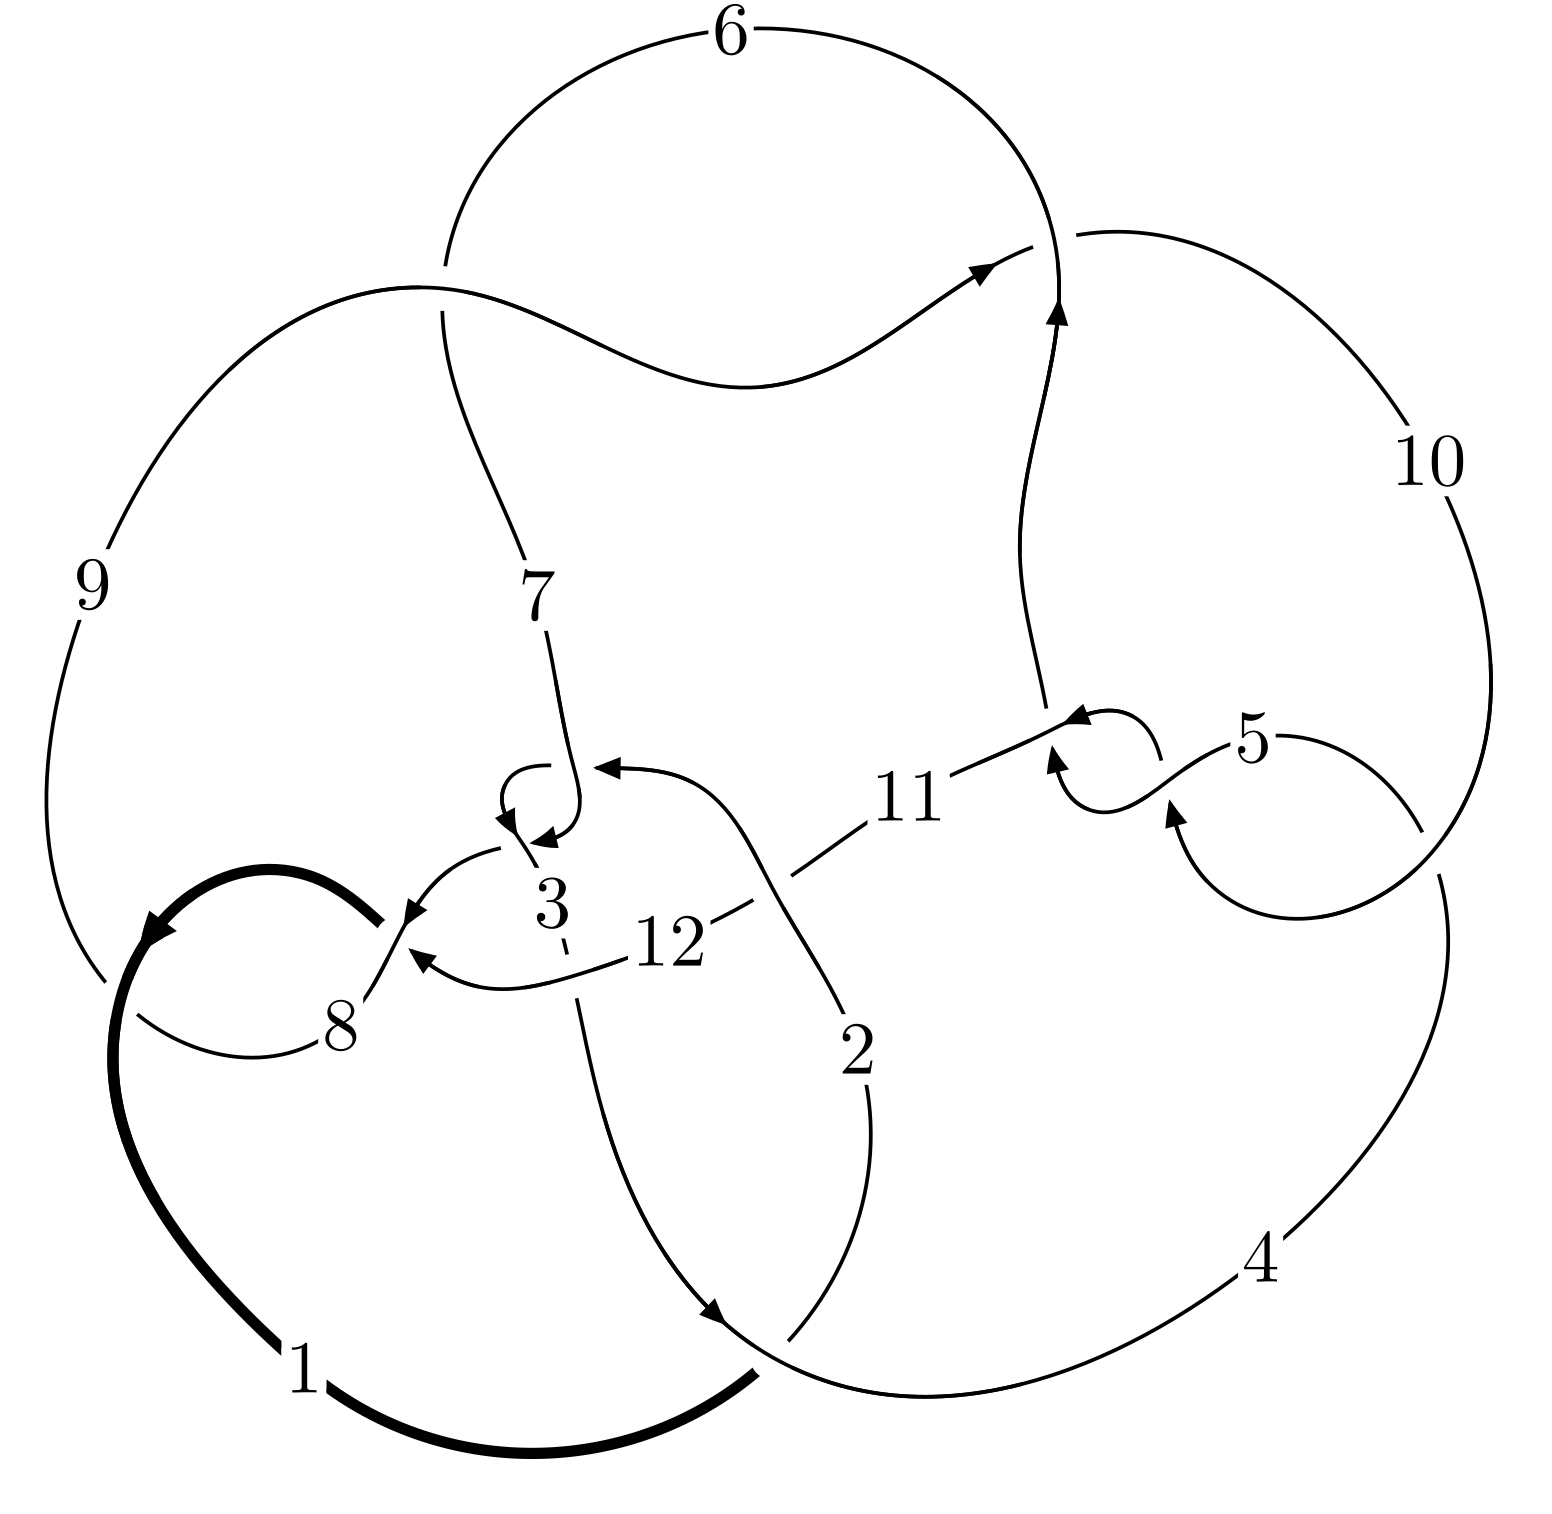
\includegraphics[width=112pt]{../../../GIT/diagram.site/Diagrams/png/1917_12a_1116.png}\\
\ \ \ A knot diagram\footnotemark}&
\allowdisplaybreaks
\textbf{Linearized knot diagam} \\
\cline{2-2}
 &
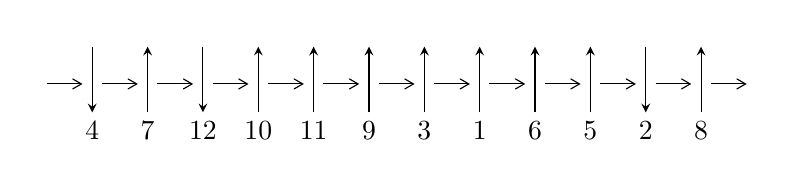
\begin{tikzpicture}[x=20pt, y=17pt]
	% nodes
	\node (C0) at (0, 0) {};
	\node (C1) at (1, 0) {};
	\node (C1U) at (1, +1) {};
	\node (C1D) at (1, -1) {4};

	\node (C2) at (2, 0) {};
	\node (C2U) at (2, +1) {};
	\node (C2D) at (2, -1) {7};

	\node (C3) at (3, 0) {};
	\node (C3U) at (3, +1) {};
	\node (C3D) at (3, -1) {12};

	\node (C4) at (4, 0) {};
	\node (C4U) at (4, +1) {};
	\node (C4D) at (4, -1) {10};

	\node (C5) at (5, 0) {};
	\node (C5U) at (5, +1) {};
	\node (C5D) at (5, -1) {11};

	\node (C6) at (6, 0) {};
	\node (C6U) at (6, +1) {};
	\node (C6D) at (6, -1) {9};

	\node (C7) at (7, 0) {};
	\node (C7U) at (7, +1) {};
	\node (C7D) at (7, -1) {3};

	\node (C8) at (8, 0) {};
	\node (C8U) at (8, +1) {};
	\node (C8D) at (8, -1) {1};

	\node (C9) at (9, 0) {};
	\node (C9U) at (9, +1) {};
	\node (C9D) at (9, -1) {6};

	\node (C10) at (10, 0) {};
	\node (C10U) at (10, +1) {};
	\node (C10D) at (10, -1) {5};

	\node (C11) at (11, 0) {};
	\node (C11U) at (11, +1) {};
	\node (C11D) at (11, -1) {2};

	\node (C12) at (12, 0) {};
	\node (C12U) at (12, +1) {};
	\node (C12D) at (12, -1) {8};
	\node (C13) at (13, 0) {};

	% arrows
	\draw[->,>={angle 60}]
	(C0) edge (C1) (C1) edge (C2) (C2) edge (C3) (C3) edge (C4) (C4) edge (C5) (C5) edge (C6) (C6) edge (C7) (C7) edge (C8) (C8) edge (C9) (C9) edge (C10) (C10) edge (C11) (C11) edge (C12) (C12) edge (C13) ;	\draw[->,>=stealth]
	(C1U) edge (C1D) (C2D) edge (C2U) (C3U) edge (C3D) (C4D) edge (C4U) (C5D) edge (C5U) (C6D) edge (C6U) (C7D) edge (C7U) (C8D) edge (C8U) (C9D) edge (C9U) (C10D) edge (C10U) (C11U) edge (C11D) (C12D) edge (C12U) ;
	\end{tikzpicture} \\
\hhline{~~} \\& 
\textbf{Solving Sequence} \\ \cline{2-2} 
 &
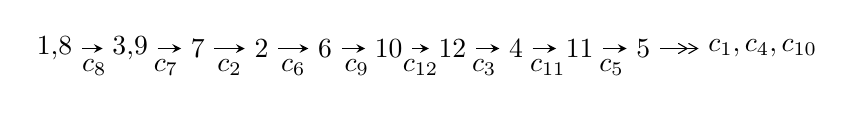
\begin{tikzpicture}[x=23pt, y=7pt]
	% node
	\node (A0) at (-1/8, 0) {1,8};
	\node (A1) at (17/16, 0) {3,9};
	\node (A2) at (17/8, 0) {7};
	\node (A3) at (25/8, 0) {2};
	\node (A4) at (33/8, 0) {6};
	\node (A5) at (41/8, 0) {10};
	\node (A6) at (49/8, 0) {12};
	\node (A7) at (57/8, 0) {4};
	\node (A8) at (65/8, 0) {11};
	\node (A9) at (73/8, 0) {5};
	\node (C1) at (1/2, -1) {$c_{8}$};
	\node (C2) at (13/8, -1) {$c_{7}$};
	\node (C3) at (21/8, -1) {$c_{2}$};
	\node (C4) at (29/8, -1) {$c_{6}$};
	\node (C5) at (37/8, -1) {$c_{9}$};
	\node (C6) at (45/8, -1) {$c_{12}$};
	\node (C7) at (53/8, -1) {$c_{3}$};
	\node (C8) at (61/8, -1) {$c_{11}$};
	\node (C9) at (69/8, -1) {$c_{5}$};
	\node (A10) at (11, 0) {$c_{1},c_{4},c_{10}$};

	% edge
	\draw[->,>=stealth]	
	(A0) edge (A1) (A1) edge (A2) (A2) edge (A3) (A3) edge (A4) (A4) edge (A5) (A5) edge (A6) (A6) edge (A7) (A7) edge (A8) (A8) edge (A9) ;
	\draw[->>,>={angle 60}]	
	(A9) edge (A10);
\end{tikzpicture} \\ 

\end{tabular} \\

\footnotetext{
The image of knot diagram is generated by the software ``\textbf{Draw programme}" developed by Andrew Bartholomew(\url{http://www.layer8.co.uk/maths/draw/index.htm\#Running-draw}), where we modified some parts for our purpose(\url{https://github.com/CATsTAILs/LinksPainter}).
}\phantom \\ \newline 
\centering \textbf{Ideals for irreducible components\footnotemark of $X_{\text{par}}$} 
 
\begin{align*}
I^u_{1}&=\langle 
b- u,\;1.05217\times10^{27} u^{39}+1.39337\times10^{27} u^{38}+\cdots+7.10616\times10^{26} a-1.70682\times10^{27},\\
\phantom{I^u_{1}}&\phantom{= \langle  }u^{40}+u^{39}+\cdots-2 u+1\rangle \\
I^u_{2}&=\langle 
-2.26032\times10^{209} u^{71}+5.90990\times10^{209} u^{70}+\cdots+4.11003\times10^{210} b-1.25850\times10^{213},\\
\phantom{I^u_{2}}&\phantom{= \langle  }-1.04624\times10^{212} u^{71}+2.60608\times10^{212} u^{70}+\cdots+1.55912\times10^{213} a-4.97927\times10^{215},\\
\phantom{I^u_{2}}&\phantom{= \langle  }u^{72}- u^{71}+\cdots-10866 u+3667\rangle \\
I^u_{3}&=\langle 
b+u,\;2 u^{19}+2 u^{18}+\cdots+a-4,\;u^{20}+u^{19}+\cdots-4 u-1\rangle \\
\\
\end{align*}
\raggedright * 3 irreducible components of $\dim_{\mathbb{C}}=0$, with total 132 representations.\\
\footnotetext{All coefficients of polynomials are rational numbers. But the coefficients are sometimes approximated in decimal forms when there is not enough margin.}
\newpage
\renewcommand{\arraystretch}{1}
\centering \section*{I. $I^u_{1}= \langle b- u,\;1.05\times10^{27} u^{39}+1.39\times10^{27} u^{38}+\cdots+7.11\times10^{26} a-1.71\times10^{27},\;u^{40}+u^{39}+\cdots-2 u+1 \rangle$}
\flushleft \textbf{(i) Arc colorings}\\
\begin{tabular}{m{7pt} m{180pt} m{7pt} m{180pt} }
\flushright $a_{1}=$&$\begin{pmatrix}0\\u\end{pmatrix}$ \\
\flushright $a_{8}=$&$\begin{pmatrix}1\\0\end{pmatrix}$ \\
\flushright $a_{3}=$&$\begin{pmatrix}-1.48065 u^{39}-1.96079 u^{38}+\cdots+1.35762 u+2.40188\\u\end{pmatrix}$ \\
\flushright $a_{9}=$&$\begin{pmatrix}1\\- u^2\end{pmatrix}$ \\
\flushright $a_{7}=$&$\begin{pmatrix}-0.480143 u^{39}-1.10267 u^{38}+\cdots-0.559408 u+2.48065\\u^2\end{pmatrix}$ \\
\flushright $a_{2}=$&$\begin{pmatrix}-0.858121 u^{39}-1.37178 u^{38}+\cdots-0.162740 u+1.92174\\- u^3+u\end{pmatrix}$ \\
\flushright $a_{6}=$&$\begin{pmatrix}-0.513657 u^{39}-0.937281 u^{38}+\cdots+0.205499 u+1.85812\\0.0881220 u^{39}-0.00106714 u^{38}+\cdots-0.431317 u+0.198901\end{pmatrix}$ \\
\flushright $a_{10}=$&$\begin{pmatrix}0.170926 u^{39}+0.314539 u^{38}+\cdots+0.337548 u+0.372176\\-0.269415 u^{39}-0.112280 u^{38}+\cdots+1.12121 u-0.412140\end{pmatrix}$ \\
\flushright $a_{12}=$&$\begin{pmatrix}- u\\u\end{pmatrix}$ \\
\flushright $a_{4}=$&$\begin{pmatrix}-0.858121 u^{39}-1.37178 u^{38}+\cdots+0.837260 u+1.92174\\-0.622525 u^{39}-0.589010 u^{38}+\cdots+1.52036 u+0.480143\end{pmatrix}$ \\
\flushright $a_{11}=$&$\begin{pmatrix}1.17203 u^{39}+1.77115 u^{38}+\cdots-0.353657 u-2.38079\\-0.313912 u^{39}-0.399375 u^{38}+\cdots+0.516397 u+0.459050\end{pmatrix}$ \\
\flushright $a_{5}=$&$\begin{pmatrix}-1.61039 u^{39}-2.45419 u^{38}+\cdots+0.621411 u+3.20931\\0.249610 u^{39}-0.0431241 u^{38}+\cdots-1.08313 u+0.723404\end{pmatrix}$\\&\end{tabular}
\flushleft \textbf{(ii) Obstruction class $= -1$}\\~\\
\flushleft \textbf{(iii) Cusp Shapes $= \frac{151015313886743544528267445}{710615561412313479871799093} u^{39}-\frac{543514532737677763668736672}{710615561412313479871799093} u^{38}+\cdots-\frac{196468822280070142794468717}{710615561412313479871799093} u+\frac{7938621198965187441158388505}{710615561412313479871799093}$}\\~\\
\newpage\renewcommand{\arraystretch}{1}
\flushleft \textbf{(iv) u-Polynomials at the component}\newline \\
\begin{tabular}{m{50pt}|m{274pt}}
Crossings & \hspace{64pt}u-Polynomials at each crossing \\
\hline $$\begin{aligned}c_{1},c_{11}\end{aligned}$$&$\begin{aligned}
&u^{40}+u^{39}+\cdots-14 u+1
\end{aligned}$\\
\hline $$\begin{aligned}c_{2},c_{7},c_{8}\\c_{12}\end{aligned}$$&$\begin{aligned}
&u^{40}+u^{39}+\cdots-2 u+1
\end{aligned}$\\
\hline $$\begin{aligned}c_{3}\end{aligned}$$&$\begin{aligned}
&u^{40}+35 u^{39}+\cdots+4063232 u+262144
\end{aligned}$\\
\hline $$\begin{aligned}c_{4},c_{5},c_{10}\end{aligned}$$&$\begin{aligned}
&u^{40}-6 u^{39}+\cdots+14 u+4
\end{aligned}$\\
\hline $$\begin{aligned}c_{6},c_{9}\end{aligned}$$&$\begin{aligned}
&u^{40}+18 u^{39}+\cdots-286 u-52
\end{aligned}$\\
\hline
\end{tabular}\\~\\
\newpage\renewcommand{\arraystretch}{1}
\flushleft \textbf{(v) Riley Polynomials at the component}\newline \\
\begin{tabular}{m{50pt}|m{274pt}}
Crossings & \hspace{64pt}Riley Polynomials at each crossing \\
\hline $$\begin{aligned}c_{1},c_{11}\end{aligned}$$&$\begin{aligned}
&y^{40}-17 y^{39}+\cdots-104 y+1
\end{aligned}$\\
\hline $$\begin{aligned}c_{2},c_{7},c_{8}\\c_{12}\end{aligned}$$&$\begin{aligned}
&y^{40}-27 y^{39}+\cdots-6 y+1
\end{aligned}$\\
\hline $$\begin{aligned}c_{3}\end{aligned}$$&$\begin{aligned}
&y^{40}-5 y^{39}+\cdots-738734374912 y+68719476736
\end{aligned}$\\
\hline $$\begin{aligned}c_{4},c_{5},c_{10}\end{aligned}$$&$\begin{aligned}
&y^{40}-34 y^{39}+\cdots-76 y+16
\end{aligned}$\\
\hline $$\begin{aligned}c_{6},c_{9}\end{aligned}$$&$\begin{aligned}
&y^{40}+22 y^{39}+\cdots-227084 y+2704
\end{aligned}$\\
\hline
\end{tabular}\\~\\
\newpage\flushleft \textbf{(vi) Complex Volumes and Cusp Shapes}
$$\begin{array}{c|c|c}  
\text{Solutions to }I^u_{1}& \I (\text{vol} + \sqrt{-1}CS) & \text{Cusp shape}\\
 \hline 
\begin{aligned}
u &= \phantom{-}0.829708 + 0.582758 I \\
a &= -0.335057 + 0.593668 I \\
b &= \phantom{-}0.829708 + 0.582758 I\end{aligned}
 & \phantom{-}0.31185 + 6.62575 I & \phantom{-}5.80735 - 6.70847 I \\ \hline\begin{aligned}
u &= \phantom{-}0.829708 - 0.582758 I \\
a &= -0.335057 - 0.593668 I \\
b &= \phantom{-}0.829708 - 0.582758 I\end{aligned}
 & \phantom{-}0.31185 - 6.62575 I & \phantom{-}5.80735 + 6.70847 I \\ \hline\begin{aligned}
u &= \phantom{-}0.950467 + 0.117799 I \\
a &= -2.79305 - 0.18733 I \\
b &= \phantom{-}0.950467 + 0.117799 I\end{aligned}
 & \phantom{-}0.479393 + 0.290586 I & \phantom{-}9.02412 - 0.47721 I \\ \hline\begin{aligned}
u &= \phantom{-}0.950467 - 0.117799 I \\
a &= -2.79305 + 0.18733 I \\
b &= \phantom{-}0.950467 - 0.117799 I\end{aligned}
 & \phantom{-}0.479393 - 0.290586 I & \phantom{-}9.02412 + 0.47721 I \\ \hline\begin{aligned}
u &= -1.045880 + 0.174408 I \\
a &= \phantom{-}2.78432 - 0.39606 I \\
b &= -1.045880 + 0.174408 I\end{aligned}
 & -1.95597 - 4.61343 I & \phantom{-}6.17888 + 5.30120 I \\ \hline\begin{aligned}
u &= -1.045880 - 0.174408 I \\
a &= \phantom{-}2.78432 + 0.39606 I \\
b &= -1.045880 - 0.174408 I\end{aligned}
 & -1.95597 + 4.61343 I & \phantom{-}6.17888 - 5.30120 I \\ \hline\begin{aligned}
u &= -1.06992\phantom{ +0.000000I} \\
a &= \phantom{-}3.35821\phantom{ +0.000000I} \\
b &= -1.06992\phantom{ +0.000000I}\end{aligned}
 & \phantom{-}8.23937\phantom{ +0.000000I} & \phantom{-}8.13250\phantom{ +0.000000I} \\ \hline\begin{aligned}
u &= -0.709739 + 0.591170 I \\
a &= \phantom{-}0.136387 + 0.470227 I \\
b &= -0.709739 + 0.591170 I\end{aligned}
 & -3.66425 - 2.23553 I & \phantom{-}2.10476 + 3.41235 I \\ \hline\begin{aligned}
u &= -0.709739 - 0.591170 I \\
a &= \phantom{-}0.136387 - 0.470227 I \\
b &= -0.709739 - 0.591170 I\end{aligned}
 & -3.66425 + 2.23553 I & \phantom{-}2.10476 - 3.41235 I \\ \hline\begin{aligned}
u &= \phantom{-}1.099650 + 0.175182 I \\
a &= -2.79566 - 0.50433 I \\
b &= \phantom{-}1.099650 + 0.175182 I\end{aligned}
 & \phantom{-}3.02582 + 8.81935 I & \phantom{-}10.62324 - 6.97053 I\\
 \hline 
 \end{array}$$\newpage$$\begin{array}{c|c|c}  
\text{Solutions to }I^u_{1}& \I (\text{vol} + \sqrt{-1}CS) & \text{Cusp shape}\\
 \hline 
\begin{aligned}
u &= \phantom{-}1.099650 - 0.175182 I \\
a &= -2.79566 + 0.50433 I \\
b &= \phantom{-}1.099650 - 0.175182 I\end{aligned}
 & \phantom{-}3.02582 - 8.81935 I & \phantom{-}10.62324 + 6.97053 I \\ \hline\begin{aligned}
u &= -0.301242 + 0.810427 I \\
a &= \phantom{-}1.231820 - 0.046364 I \\
b &= -0.301242 + 0.810427 I\end{aligned}
 & -1.68748 + 6.67297 I & \phantom{-}4.33952 - 4.30566 I \\ \hline\begin{aligned}
u &= -0.301242 - 0.810427 I \\
a &= \phantom{-}1.231820 + 0.046364 I \\
b &= -0.301242 - 0.810427 I\end{aligned}
 & -1.68748 - 6.67297 I & \phantom{-}4.33952 + 4.30566 I \\ \hline\begin{aligned}
u &= \phantom{-}0.575167 + 0.621713 I \\
a &= \phantom{-}0.009634 + 0.324370 I \\
b &= \phantom{-}0.575167 + 0.621713 I\end{aligned}
 & \phantom{-}0.17012 - 2.02828 I & \phantom{-}6.28682 - 0.18788 I \\ \hline\begin{aligned}
u &= \phantom{-}0.575167 - 0.621713 I \\
a &= \phantom{-}0.009634 - 0.324370 I \\
b &= \phantom{-}0.575167 - 0.621713 I\end{aligned}
 & \phantom{-}0.17012 + 2.02828 I & \phantom{-}6.28682 + 0.18788 I \\ \hline\begin{aligned}
u &= \phantom{-}0.347115 + 0.764028 I \\
a &= -1.348860 + 0.000533 I \\
b &= \phantom{-}0.347115 + 0.764028 I\end{aligned}
 & -5.94604 - 2.55676 I & -0.337170 + 1.059387 I \\ \hline\begin{aligned}
u &= \phantom{-}0.347115 - 0.764028 I \\
a &= -1.348860 - 0.000533 I \\
b &= \phantom{-}0.347115 - 0.764028 I\end{aligned}
 & -5.94604 + 2.55676 I & -0.337170 - 1.059387 I \\ \hline\begin{aligned}
u &= -0.408843 + 0.706524 I \\
a &= \phantom{-}1.51264 + 0.04027 I \\
b &= -0.408843 + 0.706524 I\end{aligned}
 & -2.38796 - 1.54380 I & \phantom{-}3.59940 + 3.55875 I \\ \hline\begin{aligned}
u &= -0.408843 - 0.706524 I \\
a &= \phantom{-}1.51264 - 0.04027 I \\
b &= -0.408843 - 0.706524 I\end{aligned}
 & -2.38796 + 1.54380 I & \phantom{-}3.59940 - 3.55875 I \\ \hline\begin{aligned}
u &= -0.744235\phantom{ +0.000000I} \\
a &= -1.54163\phantom{ +0.000000I} \\
b &= -0.744235\phantom{ +0.000000I}\end{aligned}
 & \phantom{-}7.13720\phantom{ +0.000000I} & \phantom{-}26.0990\phantom{ +0.000000I}\\
 \hline 
 \end{array}$$\newpage$$\begin{array}{c|c|c}  
\text{Solutions to }I^u_{1}& \I (\text{vol} + \sqrt{-1}CS) & \text{Cusp shape}\\
 \hline 
\begin{aligned}
u &= -1.233550 + 0.336291 I \\
a &= \phantom{-}1.58613 + 1.22068 I \\
b &= -1.233550 + 0.336291 I\end{aligned}
 & \phantom{-}10.81870 - 1.65128 I & \phantom{-}14.7327 + 4.5795 I \\ \hline\begin{aligned}
u &= -1.233550 - 0.336291 I \\
a &= \phantom{-}1.58613 - 1.22068 I \\
b &= -1.233550 - 0.336291 I\end{aligned}
 & \phantom{-}10.81870 + 1.65128 I & \phantom{-}14.7327 - 4.5795 I \\ \hline\begin{aligned}
u &= \phantom{-}1.230890 + 0.434304 I \\
a &= -1.40654 + 0.97624 I \\
b &= \phantom{-}1.230890 + 0.434304 I\end{aligned}
 & \phantom{-}4.92417 + 4.68998 I & \phantom{-}8.58815 - 3.67892 I \\ \hline\begin{aligned}
u &= \phantom{-}1.230890 - 0.434304 I \\
a &= -1.40654 - 0.97624 I \\
b &= \phantom{-}1.230890 - 0.434304 I\end{aligned}
 & \phantom{-}4.92417 - 4.68998 I & \phantom{-}8.58815 + 3.67892 I \\ \hline\begin{aligned}
u &= -0.008320 + 0.688792 I \\
a &= -0.644264 + 0.267316 I \\
b &= -0.008320 + 0.688792 I\end{aligned}
 & \phantom{-}3.24536 - 1.80566 I & \phantom{-}7.66277 + 3.84341 I \\ \hline\begin{aligned}
u &= -0.008320 - 0.688792 I \\
a &= -0.644264 - 0.267316 I \\
b &= -0.008320 - 0.688792 I\end{aligned}
 & \phantom{-}3.24536 + 1.80566 I & \phantom{-}7.66277 - 3.84341 I \\ \hline\begin{aligned}
u &= \phantom{-}0.619486\phantom{ +0.000000I} \\
a &= -2.75105\phantom{ +0.000000I} \\
b &= \phantom{-}0.619486\phantom{ +0.000000I}\end{aligned}
 & \phantom{-}0.329159\phantom{ +0.000000I} & \phantom{-}14.0190\phantom{ +0.000000I} \\ \hline\begin{aligned}
u &= -1.306240 + 0.490977 I \\
a &= \phantom{-}1.50397 + 0.75841 I \\
b &= -1.306240 + 0.490977 I\end{aligned}
 & \phantom{-}5.64753 - 8.73681 I & \phantom{-}9.75964 + 8.45348 I \\ \hline\begin{aligned}
u &= -1.306240 - 0.490977 I \\
a &= \phantom{-}1.50397 - 0.75841 I \\
b &= -1.306240 - 0.490977 I\end{aligned}
 & \phantom{-}5.64753 + 8.73681 I & \phantom{-}9.75964 - 8.45348 I \\ \hline\begin{aligned}
u &= \phantom{-}1.39043 + 0.46049 I \\
a &= -1.69234 + 0.71463 I \\
b &= \phantom{-}1.39043 + 0.46049 I\end{aligned}
 & \phantom{-}12.1702 + 10.4927 I & \phantom{-0.000000 } 0\\
 \hline 
 \end{array}$$\newpage$$\begin{array}{c|c|c}  
\text{Solutions to }I^u_{1}& \I (\text{vol} + \sqrt{-1}CS) & \text{Cusp shape}\\
 \hline 
\begin{aligned}
u &= \phantom{-}1.39043 - 0.46049 I \\
a &= -1.69234 - 0.71463 I \\
b &= \phantom{-}1.39043 - 0.46049 I\end{aligned}
 & \phantom{-}12.1702 - 10.4927 I & \phantom{-0.000000 } 0 \\ \hline\begin{aligned}
u &= -1.37616 + 0.58894 I \\
a &= \phantom{-}1.53982 + 0.51187 I \\
b &= -1.37616 + 0.58894 I\end{aligned}
 & \phantom{-}3.95118 - 8.98770 I & \phantom{-0.000000 } 0 \\ \hline\begin{aligned}
u &= -1.37616 - 0.58894 I \\
a &= \phantom{-}1.53982 - 0.51187 I \\
b &= -1.37616 - 0.58894 I\end{aligned}
 & \phantom{-}3.95118 + 8.98770 I & \phantom{-0.000000 } 0 \\ \hline\begin{aligned}
u &= -0.114437 + 0.486204 I \\
a &= \phantom{-}0.910358 + 0.962474 I \\
b &= -0.114437 + 0.486204 I\end{aligned}
 & -1.35206 + 0.83491 I & -2.58594 - 2.82924 I \\ \hline\begin{aligned}
u &= -0.114437 - 0.486204 I \\
a &= \phantom{-}0.910358 - 0.962474 I \\
b &= -0.114437 - 0.486204 I\end{aligned}
 & -1.35206 - 0.83491 I & -2.58594 + 2.82924 I \\ \hline\begin{aligned}
u &= \phantom{-}1.41567 + 0.59218 I \\
a &= -1.60292 + 0.47452 I \\
b &= \phantom{-}1.41567 + 0.59218 I\end{aligned}
 & \phantom{-}1.03205 + 13.48300 I & \phantom{-0.000000 } 0 \\ \hline\begin{aligned}
u &= \phantom{-}1.41567 - 0.59218 I \\
a &= -1.60292 - 0.47452 I \\
b &= \phantom{-}1.41567 - 0.59218 I\end{aligned}
 & \phantom{-}1.03205 - 13.48300 I & \phantom{-0.000000 } 0 \\ \hline\begin{aligned}
u &= -1.44142 + 0.58645 I \\
a &= \phantom{-}1.64842 + 0.46268 I \\
b &= -1.44142 + 0.58645 I\end{aligned}
 & \phantom{-}5.7710 - 17.8215 I & \phantom{-0.000000 } 0 \\ \hline\begin{aligned}
u &= -1.44142 - 0.58645 I \\
a &= \phantom{-}1.64842 - 0.46268 I \\
b &= -1.44142 - 0.58645 I\end{aligned}
 & \phantom{-}5.7710 + 17.8215 I & \phantom{-0.000000 } 0 \\ \hline\begin{aligned}
u &= \phantom{-}0.408146\phantom{ +0.000000I} \\
a &= \phantom{-}0.444839\phantom{ +0.000000I} \\
b &= \phantom{-}0.408146\phantom{ +0.000000I}\end{aligned}
 & \phantom{-}0.723836\phantom{ +0.000000I} & \phantom{-}14.2940\phantom{ +0.000000I}\\
 \hline 
 \end{array}$$\newpage\newpage\renewcommand{\arraystretch}{1}
\centering \section*{II. $I^u_{2}= \langle -2.26\times10^{209} u^{71}+5.91\times10^{209} u^{70}+\cdots+4.11\times10^{210} b-1.26\times10^{213},\;-1.05\times10^{212} u^{71}+2.61\times10^{212} u^{70}+\cdots+1.56\times10^{213} a-4.98\times10^{215},\;u^{72}- u^{71}+\cdots-10866 u+3667 \rangle$}
\flushleft \textbf{(i) Arc colorings}\\
\begin{tabular}{m{7pt} m{180pt} m{7pt} m{180pt} }
\flushright $a_{1}=$&$\begin{pmatrix}0\\u\end{pmatrix}$ \\
\flushright $a_{8}=$&$\begin{pmatrix}1\\0\end{pmatrix}$ \\
\flushright $a_{3}=$&$\begin{pmatrix}0.0671046 u^{71}-0.167151 u^{70}+\cdots-1109.95 u+319.364\\0.0549952 u^{71}-0.143792 u^{70}+\cdots-1113.13 u+306.203\end{pmatrix}$ \\
\flushright $a_{9}=$&$\begin{pmatrix}1\\- u^2\end{pmatrix}$ \\
\flushright $a_{7}=$&$\begin{pmatrix}-0.0301419 u^{71}+0.0293224 u^{70}+\cdots+395.244 u-87.4100\\0.328648 u^{71}-0.521975 u^{70}+\cdots-3059.47 u+668.529\end{pmatrix}$ \\
\flushright $a_{2}=$&$\begin{pmatrix}0.278968 u^{71}-0.729274 u^{70}+\cdots-5396.58 u+1506.02\\-0.454216 u^{71}+1.22463 u^{70}+\cdots+8943.08 u-2530.76\end{pmatrix}$ \\
\flushright $a_{6}=$&$\begin{pmatrix}-0.339538 u^{71}+0.567129 u^{70}+\cdots+3353.09 u-758.945\\0.688383 u^{71}-1.16484 u^{70}+\cdots-6675.94 u+1506.11\end{pmatrix}$ \\
\flushright $a_{10}=$&$\begin{pmatrix}0.541344 u^{71}-0.890028 u^{70}+\cdots-4490.24 u+952.255\\-0.342960 u^{71}+0.537379 u^{70}+\cdots+2175.57 u-399.573\end{pmatrix}$ \\
\flushright $a_{12}=$&$\begin{pmatrix}- u\\u\end{pmatrix}$ \\
\flushright $a_{4}=$&$\begin{pmatrix}-0.0741667 u^{71}+0.182756 u^{70}+\cdots+1389.76 u-373.122\\0.196267 u^{71}-0.493699 u^{70}+\cdots-3612.84 u+998.690\end{pmatrix}$ \\
\flushright $a_{11}=$&$\begin{pmatrix}0.447909 u^{71}-1.21674 u^{70}+\cdots-8536.05 u+2445.31\\-0.367683 u^{71}+1.02998 u^{70}+\cdots+7199.69 u-2091.60\end{pmatrix}$ \\
\flushright $a_{5}=$&$\begin{pmatrix}0.621670 u^{71}-1.32742 u^{70}+\cdots-8696.78 u+2258.81\\-0.208971 u^{71}+0.514036 u^{70}+\cdots+3370.06 u-922.984\end{pmatrix}$\\&\end{tabular}
\flushleft \textbf{(ii) Obstruction class $= -1$}\\~\\
\flushleft \textbf{(iii) Cusp Shapes $= 0.552929 u^{71}-1.11719 u^{70}+\cdots-7329.04 u+1860.11$}\\~\\
\newpage\renewcommand{\arraystretch}{1}
\flushleft \textbf{(iv) u-Polynomials at the component}\newline \\
\begin{tabular}{m{50pt}|m{274pt}}
Crossings & \hspace{64pt}u-Polynomials at each crossing \\
\hline $$\begin{aligned}c_{1},c_{11}\end{aligned}$$&$\begin{aligned}
&u^{72}-19 u^{71}+\cdots+178 u+13
\end{aligned}$\\
\hline $$\begin{aligned}c_{2},c_{7},c_{8}\\c_{12}\end{aligned}$$&$\begin{aligned}
&u^{72}- u^{71}+\cdots-10866 u+3667
\end{aligned}$\\
\hline $$\begin{aligned}c_{3}\end{aligned}$$&$\begin{aligned}
&(u^2- u+1)^{36}
\end{aligned}$\\
\hline $$\begin{aligned}c_{4},c_{5},c_{10}\end{aligned}$$&$\begin{aligned}
&(u^{18}+u^{17}+\cdots- u-1)^{4}
\end{aligned}$\\
\hline $$\begin{aligned}c_{6},c_{9}\end{aligned}$$&$\begin{aligned}
&(u^{18}-3 u^{17}+\cdots-3 u+3)^{4}
\end{aligned}$\\
\hline
\end{tabular}\\~\\
\newpage\renewcommand{\arraystretch}{1}
\flushleft \textbf{(v) Riley Polynomials at the component}\newline \\
\begin{tabular}{m{50pt}|m{274pt}}
Crossings & \hspace{64pt}Riley Polynomials at each crossing \\
\hline $$\begin{aligned}c_{1},c_{11}\end{aligned}$$&$\begin{aligned}
&y^{72}+11 y^{71}+\cdots-11560 y+169
\end{aligned}$\\
\hline $$\begin{aligned}c_{2},c_{7},c_{8}\\c_{12}\end{aligned}$$&$\begin{aligned}
&y^{72}-57 y^{71}+\cdots-103020588 y+13446889
\end{aligned}$\\
\hline $$\begin{aligned}c_{3}\end{aligned}$$&$\begin{aligned}
&(y^2+y+1)^{36}
\end{aligned}$\\
\hline $$\begin{aligned}c_{4},c_{5},c_{10}\end{aligned}$$&$\begin{aligned}
&(y^{18}-15 y^{17}+\cdots-7 y+1)^{4}
\end{aligned}$\\
\hline $$\begin{aligned}c_{6},c_{9}\end{aligned}$$&$\begin{aligned}
&(y^{18}+13 y^{17}+\cdots-75 y+9)^{4}
\end{aligned}$\\
\hline
\end{tabular}\\~\\
\newpage\flushleft \textbf{(vi) Complex Volumes and Cusp Shapes}
$$\begin{array}{c|c|c}  
\text{Solutions to }I^u_{2}& \I (\text{vol} + \sqrt{-1}CS) & \text{Cusp shape}\\
 \hline 
\begin{aligned}
u &= \phantom{-}1.017220 + 0.027464 I \\
a &= \phantom{-}2.13206 - 0.52858 I \\
b &= -1.66385 - 0.33543 I\end{aligned}
 & \phantom{-}2.50861 + 0.14420 I & \phantom{-0.000000 } 0 \\ \hline\begin{aligned}
u &= \phantom{-}1.017220 - 0.027464 I \\
a &= \phantom{-}2.13206 + 0.52858 I \\
b &= -1.66385 + 0.33543 I\end{aligned}
 & \phantom{-}2.50861 - 0.14420 I & \phantom{-0.000000 } 0 \\ \hline\begin{aligned}
u &= \phantom{-}0.693662 + 0.751370 I \\
a &= \phantom{-}0.303778 + 0.388548 I \\
b &= \phantom{-}0.650141 - 0.173344 I\end{aligned}
 & -0.21034 - 1.47092 I & \phantom{-0.000000 } 0 \\ \hline\begin{aligned}
u &= \phantom{-}0.693662 - 0.751370 I \\
a &= \phantom{-}0.303778 - 0.388548 I \\
b &= \phantom{-}0.650141 + 0.173344 I\end{aligned}
 & -0.21034 + 1.47092 I & \phantom{-0.000000 } 0 \\ \hline\begin{aligned}
u &= \phantom{-}1.033500 + 0.072324 I \\
a &= \phantom{-}0.293773 - 0.211699 I \\
b &= \phantom{-}0.129307 - 0.655859 I\end{aligned}
 & \phantom{-}1.58118 + 0.45801 I & \phantom{-0.000000 } 0 \\ \hline\begin{aligned}
u &= \phantom{-}1.033500 - 0.072324 I \\
a &= \phantom{-}0.293773 + 0.211699 I \\
b &= \phantom{-}0.129307 + 0.655859 I\end{aligned}
 & \phantom{-}1.58118 - 0.45801 I & \phantom{-0.000000 } 0 \\ \hline\begin{aligned}
u &= \phantom{-}0.031660 + 0.944468 I \\
a &= \phantom{-}0.220232 - 0.330295 I \\
b &= -1.118420 - 0.229212 I\end{aligned}
 & \phantom{-}1.58118 + 3.60176 I & \phantom{-0.000000 } 0. - 7.68480 I \\ \hline\begin{aligned}
u &= \phantom{-}0.031660 - 0.944468 I \\
a &= \phantom{-}0.220232 + 0.330295 I \\
b &= -1.118420 + 0.229212 I\end{aligned}
 & \phantom{-}1.58118 - 3.60176 I & \phantom{-0.000000 -}0. + 7.68480 I \\ \hline\begin{aligned}
u &= -1.066340 + 0.019440 I \\
a &= -2.19706 + 0.41240 I \\
b &= \phantom{-}1.71352 + 0.39093 I\end{aligned}
 & \phantom{-}6.82360 - 3.68439 I & \phantom{-0.000000 } 0 \\ \hline\begin{aligned}
u &= -1.066340 - 0.019440 I \\
a &= -2.19706 - 0.41240 I \\
b &= \phantom{-}1.71352 - 0.39093 I\end{aligned}
 & \phantom{-}6.82360 + 3.68439 I & \phantom{-0.000000 } 0\\
 \hline 
 \end{array}$$\newpage$$\begin{array}{c|c|c}  
\text{Solutions to }I^u_{2}& \I (\text{vol} + \sqrt{-1}CS) & \text{Cusp shape}\\
 \hline 
\begin{aligned}
u &= -0.913482 + 0.085334 I \\
a &= -2.06764 - 0.75190 I \\
b &= \phantom{-}1.61282 - 0.23864 I\end{aligned}
 & \phantom{-}6.06357 - 3.81683 I & \phantom{-}11.23943 + 0. I\phantom{ +0.000000I} \\ \hline\begin{aligned}
u &= -0.913482 - 0.085334 I \\
a &= -2.06764 + 0.75190 I \\
b &= \phantom{-}1.61282 + 0.23864 I\end{aligned}
 & \phantom{-}6.06357 + 3.81683 I & \phantom{-}11.23943 + 0. I\phantom{ +0.000000I} \\ \hline\begin{aligned}
u &= -0.846987 + 0.697488 I \\
a &= -0.333673 + 0.483654 I \\
b &= -0.519849 - 0.164047 I\end{aligned}
 & -3.45249 - 2.84406 I & \phantom{-0.000000 } 0 \\ \hline\begin{aligned}
u &= -0.846987 - 0.697488 I \\
a &= -0.333673 - 0.483654 I \\
b &= -0.519849 + 0.164047 I\end{aligned}
 & -3.45249 + 2.84406 I & \phantom{-0.000000 } 0 \\ \hline\begin{aligned}
u &= -0.289505 + 1.062300 I \\
a &= -0.594187 - 0.376086 I \\
b &= \phantom{-}1.233660 - 0.268864 I\end{aligned}
 & \phantom{-}7.08808 - 5.25662 I & \phantom{-0.000000 } 0 \\ \hline\begin{aligned}
u &= -0.289505 - 1.062300 I \\
a &= -0.594187 + 0.376086 I \\
b &= \phantom{-}1.233660 + 0.268864 I\end{aligned}
 & \phantom{-}7.08808 + 5.25662 I & \phantom{-0.000000 } 0 \\ \hline\begin{aligned}
u &= -1.118420 + 0.229212 I \\
a &= -0.308403 + 0.113424 I \\
b &= \phantom{-}0.031660 - 0.944468 I\end{aligned}
 & \phantom{-}1.58118 - 3.60176 I & \phantom{-0.000000 } 0 \\ \hline\begin{aligned}
u &= -1.118420 - 0.229212 I \\
a &= -0.308403 - 0.113424 I \\
b &= \phantom{-}0.031660 + 0.944468 I\end{aligned}
 & \phantom{-}1.58118 + 3.60176 I & \phantom{-0.000000 } 0 \\ \hline\begin{aligned}
u &= \phantom{-}0.955436 + 0.668372 I \\
a &= \phantom{-}0.353081 + 0.532513 I \\
b &= \phantom{-}0.424031 - 0.169720 I\end{aligned}
 & \phantom{-}1.04456 + 7.10521 I & \phantom{-0.000000 } 0 \\ \hline\begin{aligned}
u &= \phantom{-}0.955436 - 0.668372 I \\
a &= \phantom{-}0.353081 - 0.532513 I \\
b &= \phantom{-}0.424031 + 0.169720 I\end{aligned}
 & \phantom{-}1.04456 - 7.10521 I & \phantom{-0.000000 } 0\\
 \hline 
 \end{array}$$\newpage$$\begin{array}{c|c|c}  
\text{Solutions to }I^u_{2}& \I (\text{vol} + \sqrt{-1}CS) & \text{Cusp shape}\\
 \hline 
\begin{aligned}
u &= -1.098140 + 0.393816 I \\
a &= -0.078496 + 0.425133 I \\
b &= -0.074344 - 1.268570 I\end{aligned}
 & -0.21034 - 2.58885 I & \phantom{-0.000000 } 0 \\ \hline\begin{aligned}
u &= -1.098140 - 0.393816 I \\
a &= -0.078496 - 0.425133 I \\
b &= -0.074344 + 1.268570 I\end{aligned}
 & -0.21034 + 2.58885 I & \phantom{-0.000000 } 0 \\ \hline\begin{aligned}
u &= -1.187800 + 0.128492 I \\
a &= -0.522626 + 0.383206 I \\
b &= \phantom{-}0.028590 + 0.292450 I\end{aligned}
 & \phantom{-}7.08808 - 1.19685 I & \phantom{-0.000000 } 0 \\ \hline\begin{aligned}
u &= -1.187800 - 0.128492 I \\
a &= -0.522626 - 0.383206 I \\
b &= \phantom{-}0.028590 - 0.292450 I\end{aligned}
 & \phantom{-}7.08808 + 1.19685 I & \phantom{-0.000000 } 0 \\ \hline\begin{aligned}
u &= \phantom{-}1.137940 + 0.411255 I \\
a &= \phantom{-}0.137911 + 0.514671 I \\
b &= \phantom{-}0.007450 - 1.328250 I\end{aligned}
 & -3.45249 + 6.90382 I & \phantom{-0.000000 } 0 \\ \hline\begin{aligned}
u &= \phantom{-}1.137940 - 0.411255 I \\
a &= \phantom{-}0.137911 - 0.514671 I \\
b &= \phantom{-}0.007450 + 1.328250 I\end{aligned}
 & -3.45249 - 6.90382 I & \phantom{-0.000000 } 0 \\ \hline\begin{aligned}
u &= -1.224820 + 0.174181 I \\
a &= -1.71777 - 0.24428 I \\
b &= \phantom{-}1.41620 - 0.50567 I\end{aligned}
 & \phantom{-}5.55672 - 2.02988 I & \phantom{-0.000000 } 0 \\ \hline\begin{aligned}
u &= -1.224820 - 0.174181 I \\
a &= -1.71777 + 0.24428 I \\
b &= \phantom{-}1.41620 + 0.50567 I\end{aligned}
 & \phantom{-}5.55672 + 2.02988 I & \phantom{-0.000000 } 0 \\ \hline\begin{aligned}
u &= -1.166860 + 0.418865 I \\
a &= -0.188865 + 0.570472 I \\
b &= \phantom{-}0.045286 - 1.364190 I\end{aligned}
 & \phantom{-}1.04456 - 11.16500 I & \phantom{-0.000000 } 0 \\ \hline\begin{aligned}
u &= -1.166860 - 0.418865 I \\
a &= -0.188865 - 0.570472 I \\
b &= \phantom{-}0.045286 + 1.364190 I\end{aligned}
 & \phantom{-}1.04456 + 11.16500 I & \phantom{-0.000000 } 0\\
 \hline 
 \end{array}$$\newpage$$\begin{array}{c|c|c}  
\text{Solutions to }I^u_{2}& \I (\text{vol} + \sqrt{-1}CS) & \text{Cusp shape}\\
 \hline 
\begin{aligned}
u &= \phantom{-}1.248510 + 0.052716 I \\
a &= \phantom{-}1.95056 - 0.08236 I \\
b &= -1.58003 - 0.62693 I\end{aligned}
 & \phantom{-}10.76740 + 2.02988 I & \phantom{-0.000000 } 0 \\ \hline\begin{aligned}
u &= \phantom{-}1.248510 - 0.052716 I \\
a &= \phantom{-}1.95056 + 0.08236 I \\
b &= -1.58003 + 0.62693 I\end{aligned}
 & \phantom{-}10.76740 - 2.02988 I & \phantom{-0.000000 } 0 \\ \hline\begin{aligned}
u &= \phantom{-}1.233660 + 0.268864 I \\
a &= \phantom{-}0.530370 + 0.307807 I \\
b &= -0.289505 - 1.062300 I\end{aligned}
 & \phantom{-}7.08808 + 5.25662 I & \phantom{-0.000000 } 0 \\ \hline\begin{aligned}
u &= \phantom{-}1.233660 - 0.268864 I \\
a &= \phantom{-}0.530370 - 0.307807 I \\
b &= -0.289505 + 1.062300 I\end{aligned}
 & \phantom{-}7.08808 - 5.25662 I & \phantom{-0.000000 } 0 \\ \hline\begin{aligned}
u &= -0.074344 + 1.268570 I \\
a &= \phantom{-}0.394783 + 0.040892 I \\
b &= -1.098140 - 0.393816 I\end{aligned}
 & -0.21034 + 2.58885 I & \phantom{-0.000000 } 0 \\ \hline\begin{aligned}
u &= -0.074344 - 1.268570 I \\
a &= \phantom{-}0.394783 - 0.040892 I \\
b &= -1.098140 + 0.393816 I\end{aligned}
 & -0.21034 - 2.58885 I & \phantom{-0.000000 } 0 \\ \hline\begin{aligned}
u &= \phantom{-}0.650141 + 0.173344 I \\
a &= -0.307229 - 0.683719 I \\
b &= \phantom{-}0.693662 - 0.751370 I\end{aligned}
 & -0.21034 + 1.47092 I & \phantom{-}7.51114 - 3.72400 I \\ \hline\begin{aligned}
u &= \phantom{-}0.650141 - 0.173344 I \\
a &= -0.307229 + 0.683719 I \\
b &= \phantom{-}0.693662 + 0.751370 I\end{aligned}
 & -0.21034 - 1.47092 I & \phantom{-}7.51114 + 3.72400 I \\ \hline\begin{aligned}
u &= \phantom{-}0.007450 + 1.328250 I \\
a &= -0.483846 + 0.038488 I \\
b &= \phantom{-}1.137940 - 0.411255 I\end{aligned}
 & -3.45249 - 6.90382 I & \phantom{-0.000000 } 0 \\ \hline\begin{aligned}
u &= \phantom{-}0.007450 - 1.328250 I \\
a &= -0.483846 - 0.038488 I \\
b &= \phantom{-}1.137940 + 0.411255 I\end{aligned}
 & -3.45249 + 6.90382 I & \phantom{-0.000000 } 0\\
 \hline 
 \end{array}$$\newpage$$\begin{array}{c|c|c}  
\text{Solutions to }I^u_{2}& \I (\text{vol} + \sqrt{-1}CS) & \text{Cusp shape}\\
 \hline 
\begin{aligned}
u &= \phantom{-}0.129307 + 0.655859 I \\
a &= \phantom{-}0.382215 - 0.410916 I \\
b &= \phantom{-}1.033500 - 0.072324 I\end{aligned}
 & \phantom{-}1.58118 - 0.45801 I & \phantom{-}7.80878 - 0.75660 I \\ \hline\begin{aligned}
u &= \phantom{-}0.129307 - 0.655859 I \\
a &= \phantom{-}0.382215 + 0.410916 I \\
b &= \phantom{-}1.033500 + 0.072324 I\end{aligned}
 & \phantom{-}1.58118 + 0.45801 I & \phantom{-}7.80878 + 0.75660 I \\ \hline\begin{aligned}
u &= \phantom{-}0.045286 + 1.364190 I \\
a &= \phantom{-}0.544891 + 0.031701 I \\
b &= -1.166860 - 0.418865 I\end{aligned}
 & \phantom{-}1.04456 + 11.16500 I & \phantom{-0.000000 } 0 \\ \hline\begin{aligned}
u &= \phantom{-}0.045286 - 1.364190 I \\
a &= \phantom{-}0.544891 - 0.031701 I \\
b &= -1.166860 + 0.418865 I\end{aligned}
 & \phantom{-}1.04456 - 11.16500 I & \phantom{-0.000000 } 0 \\ \hline\begin{aligned}
u &= \phantom{-}1.370090 + 0.136727 I \\
a &= \phantom{-}1.61237 + 0.18879 I \\
b &= -1.31349 - 0.85071 I\end{aligned}
 & \phantom{-}2.50861 + 3.91557 I & \phantom{-0.000000 } 0 \\ \hline\begin{aligned}
u &= \phantom{-}1.370090 - 0.136727 I \\
a &= \phantom{-}1.61237 - 0.18879 I \\
b &= -1.31349 + 0.85071 I\end{aligned}
 & \phantom{-}2.50861 - 3.91557 I & \phantom{-0.000000 } 0 \\ \hline\begin{aligned}
u &= -1.372800 + 0.107076 I \\
a &= -1.71771 + 0.21747 I \\
b &= \phantom{-}1.40460 - 0.87274 I\end{aligned}
 & \phantom{-}6.82360 - 7.74416 I & \phantom{-0.000000 } 0 \\ \hline\begin{aligned}
u &= -1.372800 - 0.107076 I \\
a &= -1.71771 - 0.21747 I \\
b &= \phantom{-}1.40460 + 0.87274 I\end{aligned}
 & \phantom{-}6.82360 + 7.74416 I & \phantom{-0.000000 } 0 \\ \hline\begin{aligned}
u &= -1.377880 + 0.171851 I \\
a &= -1.44111 + 0.19069 I \\
b &= \phantom{-}1.16098 - 0.85415 I\end{aligned}
 & \phantom{-}6.06357 - 0.24294 I & \phantom{-0.000000 } 0 \\ \hline\begin{aligned}
u &= -1.377880 - 0.171851 I \\
a &= -1.44111 - 0.19069 I \\
b &= \phantom{-}1.16098 + 0.85415 I\end{aligned}
 & \phantom{-}6.06357 + 0.24294 I & \phantom{-0.000000 } 0\\
 \hline 
 \end{array}$$\newpage$$\begin{array}{c|c|c}  
\text{Solutions to }I^u_{2}& \I (\text{vol} + \sqrt{-1}CS) & \text{Cusp shape}\\
 \hline 
\begin{aligned}
u &= \phantom{-}1.16098 + 0.85415 I \\
a &= \phantom{-}1.301240 - 0.517704 I \\
b &= -1.377880 - 0.171851 I\end{aligned}
 & \phantom{-}6.06357 + 0.24294 I & \phantom{-0.000000 } 0 \\ \hline\begin{aligned}
u &= \phantom{-}1.16098 - 0.85415 I \\
a &= \phantom{-}1.301240 + 0.517704 I \\
b &= -1.377880 + 0.171851 I\end{aligned}
 & \phantom{-}6.06357 - 0.24294 I & \phantom{-0.000000 } 0 \\ \hline\begin{aligned}
u &= -0.519849 + 0.164047 I \\
a &= \phantom{-}0.450371 - 1.093590 I \\
b &= -0.846987 - 0.697488 I\end{aligned}
 & -3.45249 + 2.84406 I & \phantom{-}4.47320 - 0.13726 I \\ \hline\begin{aligned}
u &= -0.519849 - 0.164047 I \\
a &= \phantom{-}0.450371 + 1.093590 I \\
b &= -0.846987 + 0.697488 I\end{aligned}
 & -3.45249 - 2.84406 I & \phantom{-}4.47320 + 0.13726 I \\ \hline\begin{aligned}
u &= \phantom{-}1.41620 + 0.50567 I \\
a &= \phantom{-}1.34430 - 0.47999 I \\
b &= -1.224820 - 0.174181 I\end{aligned}
 & \phantom{-}5.55672 + 2.02988 I & \phantom{-0.000000 } 0 \\ \hline\begin{aligned}
u &= \phantom{-}1.41620 - 0.50567 I \\
a &= \phantom{-}1.34430 + 0.47999 I \\
b &= -1.224820 + 0.174181 I\end{aligned}
 & \phantom{-}5.55672 - 2.02988 I & \phantom{-0.000000 } 0 \\ \hline\begin{aligned}
u &= \phantom{-}0.424031 + 0.169720 I \\
a &= -0.64369 - 1.49877 I \\
b &= \phantom{-}0.955436 - 0.668372 I\end{aligned}
 & \phantom{-}1.04456 - 7.10521 I & \phantom{-}8.98695 + 2.40068 I \\ \hline\begin{aligned}
u &= \phantom{-}0.424031 - 0.169720 I \\
a &= -0.64369 + 1.49877 I \\
b &= \phantom{-}0.955436 + 0.668372 I\end{aligned}
 & \phantom{-}1.04456 + 7.10521 I & \phantom{-}8.98695 - 2.40068 I \\ \hline\begin{aligned}
u &= -1.31349 + 0.85071 I \\
a &= -1.33743 - 0.50145 I \\
b &= \phantom{-}1.370090 - 0.136727 I\end{aligned}
 & \phantom{-}2.50861 - 3.91557 I & \phantom{-0.000000 } 0 \\ \hline\begin{aligned}
u &= -1.31349 - 0.85071 I \\
a &= -1.33743 + 0.50145 I \\
b &= \phantom{-}1.370090 + 0.136727 I\end{aligned}
 & \phantom{-}2.50861 + 3.91557 I & \phantom{-0.000000 } 0\\
 \hline 
 \end{array}$$\newpage$$\begin{array}{c|c|c}  
\text{Solutions to }I^u_{2}& \I (\text{vol} + \sqrt{-1}CS) & \text{Cusp shape}\\
 \hline 
\begin{aligned}
u &= \phantom{-}1.61282 + 0.23864 I \\
a &= \phantom{-}1.139110 - 0.485015 I \\
b &= -0.913482 - 0.085334 I\end{aligned}
 & \phantom{-}6.06357 + 3.81683 I & \phantom{-0.000000 } 0 \\ \hline\begin{aligned}
u &= \phantom{-}1.61282 - 0.23864 I \\
a &= \phantom{-}1.139110 + 0.485015 I \\
b &= -0.913482 + 0.085334 I\end{aligned}
 & \phantom{-}6.06357 - 3.81683 I & \phantom{-0.000000 } 0 \\ \hline\begin{aligned}
u &= \phantom{-}1.40460 + 0.87274 I \\
a &= \phantom{-}1.35323 - 0.49733 I \\
b &= -1.372800 - 0.107076 I\end{aligned}
 & \phantom{-}6.82360 + 7.74416 I & \phantom{-0.000000 } 0 \\ \hline\begin{aligned}
u &= \phantom{-}1.40460 - 0.87274 I \\
a &= \phantom{-}1.35323 + 0.49733 I \\
b &= -1.372800 + 0.107076 I\end{aligned}
 & \phantom{-}6.82360 - 7.74416 I & \phantom{-0.000000 } 0 \\ \hline\begin{aligned}
u &= -1.66385 + 0.33543 I \\
a &= -1.205150 - 0.530920 I \\
b &= \phantom{-}1.017220 - 0.027464 I\end{aligned}
 & \phantom{-}2.50861 - 0.14420 I & \phantom{-0.000000 } 0 \\ \hline\begin{aligned}
u &= -1.66385 - 0.33543 I \\
a &= -1.205150 + 0.530920 I \\
b &= \phantom{-}1.017220 + 0.027464 I\end{aligned}
 & \phantom{-}2.50861 + 0.14420 I & \phantom{-0.000000 } 0 \\ \hline\begin{aligned}
u &= -1.58003 + 0.62693 I \\
a &= -1.33401 - 0.52932 I \\
b &= \phantom{-}1.248510 - 0.052716 I\end{aligned}
 & \phantom{-}10.76740 - 2.02988 I & \phantom{-0.000000 } 0 \\ \hline\begin{aligned}
u &= -1.58003 - 0.62693 I \\
a &= -1.33401 + 0.52932 I \\
b &= \phantom{-}1.248510 + 0.052716 I\end{aligned}
 & \phantom{-}10.76740 + 2.02988 I & \phantom{-0.000000 } 0 \\ \hline\begin{aligned}
u &= \phantom{-}0.028590 + 0.292450 I \\
a &= -1.57989 - 2.10875 I \\
b &= -1.187800 + 0.128492 I\end{aligned}
 & \phantom{-}7.08808 - 1.19685 I & \phantom{-}13.05526 + 0.16546 I \\ \hline\begin{aligned}
u &= \phantom{-}0.028590 - 0.292450 I \\
a &= -1.57989 + 2.10875 I \\
b &= -1.187800 - 0.128492 I\end{aligned}
 & \phantom{-}7.08808 + 1.19685 I & \phantom{-}13.05526 - 0.16546 I\\
 \hline 
 \end{array}$$\newpage$$\begin{array}{c|c|c}  
\text{Solutions to }I^u_{2}& \I (\text{vol} + \sqrt{-1}CS) & \text{Cusp shape}\\
 \hline 
\begin{aligned}
u &= \phantom{-}1.71352 + 0.39093 I \\
a &= \phantom{-}1.234100 - 0.563121 I \\
b &= -1.066340 + 0.019440 I\end{aligned}
 & \phantom{-}6.82360 - 3.68439 I & \phantom{-0.000000 } 0 \\ \hline\begin{aligned}
u &= \phantom{-}1.71352 - 0.39093 I \\
a &= \phantom{-}1.234100 + 0.563121 I \\
b &= -1.066340 - 0.019440 I\end{aligned}
 & \phantom{-}6.82360 + 3.68439 I & \phantom{-0.000000 } 0\\
 \hline 
 \end{array}$$\newpage\newpage\renewcommand{\arraystretch}{1}
\centering \section*{III. $I^u_{3}= \langle b+u,\;2 u^{19}+2 u^{18}+\cdots+a-4,\;u^{20}+u^{19}+\cdots-4 u-1 \rangle$}
\flushleft \textbf{(i) Arc colorings}\\
\begin{tabular}{m{7pt} m{180pt} m{7pt} m{180pt} }
\flushright $a_{1}=$&$\begin{pmatrix}0\\u\end{pmatrix}$ \\
\flushright $a_{8}=$&$\begin{pmatrix}1\\0\end{pmatrix}$ \\
\flushright $a_{3}=$&$\begin{pmatrix}-2 u^{19}-2 u^{18}+\cdots-3 u+4\\- u\end{pmatrix}$ \\
\flushright $a_{9}=$&$\begin{pmatrix}1\\- u^2\end{pmatrix}$ \\
\flushright $a_{7}=$&$\begin{pmatrix}u^{18}+u^{17}+\cdots+4 u+3\\u^2\end{pmatrix}$ \\
\flushright $a_{2}=$&$\begin{pmatrix}- u^{19}- u^{18}+\cdots-23 u^2+4\\u^3- u\end{pmatrix}$ \\
\flushright $a_{6}=$&$\begin{pmatrix}u^4-3 u^2+2\\u^{18}+u^{17}+\cdots+4 u+1\end{pmatrix}$ \\
\flushright $a_{10}=$&$\begin{pmatrix}u^8-5 u^6+9 u^4-6 u^2+1\\- u^{18}- u^{17}+\cdots-8 u-2\end{pmatrix}$ \\
\flushright $a_{12}=$&$\begin{pmatrix}- u\\u\end{pmatrix}$ \\
\flushright $a_{4}=$&$\begin{pmatrix}- u^{19}- u^{18}+\cdots- u+4\\- u^{19}- u^{18}+\cdots-4 u^2-3 u\end{pmatrix}$ \\
\flushright $a_{11}=$&$\begin{pmatrix}u^{19}+u^{18}+\cdots-2 u-4\\u^5-2 u^3+2 u\end{pmatrix}$ \\
\flushright $a_{5}=$&$\begin{pmatrix}- u^{18}- u^{17}+\cdots-4 u+4\\2 u^{18}+2 u^{17}+\cdots+8 u+2\end{pmatrix}$\\&\end{tabular}
\flushleft \textbf{(ii) Obstruction class $= 1$}\\~\\
\flushleft \textbf{(iii) Cusp Shapes $= - u^{19}-7 u^{18}+3 u^{17}+65 u^{16}+20 u^{15}-268 u^{14}-151 u^{13}+623 u^{12}+438 u^{11}-868 u^{10}-705 u^9+708 u^8+674 u^7-305 u^6-385 u^5+57 u^4+140 u^3-34 u-7$}\\~\\
\newpage\renewcommand{\arraystretch}{1}
\flushleft \textbf{(iv) u-Polynomials at the component}\newline \\
\begin{tabular}{m{50pt}|m{274pt}}
Crossings & \hspace{64pt}u-Polynomials at each crossing \\
\hline $$\begin{aligned}c_{1},c_{11}\end{aligned}$$&$\begin{aligned}
&u^{20}+u^{19}+\cdots-2 u+1
\end{aligned}$\\
\hline $$\begin{aligned}c_{2},c_{8}\end{aligned}$$&$\begin{aligned}
&u^{20}+u^{19}+\cdots-4 u-1
\end{aligned}$\\
\hline $$\begin{aligned}c_{3}\end{aligned}$$&$\begin{aligned}
&u^{20}+2 u^{19}+\cdots- u+1
\end{aligned}$\\
\hline $$\begin{aligned}c_{4},c_{5}\end{aligned}$$&$\begin{aligned}
&u^{20}- u^{19}+\cdots+u-1
\end{aligned}$\\
\hline $$\begin{aligned}c_{6}\end{aligned}$$&$\begin{aligned}
&u^{20}+3 u^{19}+\cdots+3 u+1
\end{aligned}$\\
\hline $$\begin{aligned}c_{7},c_{12}\end{aligned}$$&$\begin{aligned}
&u^{20}- u^{19}+\cdots+4 u-1
\end{aligned}$\\
\hline $$\begin{aligned}c_{9}\end{aligned}$$&$\begin{aligned}
&u^{20}-3 u^{19}+\cdots-3 u+1
\end{aligned}$\\
\hline $$\begin{aligned}c_{10}\end{aligned}$$&$\begin{aligned}
&u^{20}+u^{19}+\cdots- u-1
\end{aligned}$\\
\hline
\end{tabular}\\~\\
\newpage\renewcommand{\arraystretch}{1}
\flushleft \textbf{(v) Riley Polynomials at the component}\newline \\
\begin{tabular}{m{50pt}|m{274pt}}
Crossings & \hspace{64pt}Riley Polynomials at each crossing \\
\hline $$\begin{aligned}c_{1},c_{11}\end{aligned}$$&$\begin{aligned}
&y^{20}+y^{19}+\cdots-6 y+1
\end{aligned}$\\
\hline $$\begin{aligned}c_{2},c_{7},c_{8}\\c_{12}\end{aligned}$$&$\begin{aligned}
&y^{20}-21 y^{19}+\cdots-20 y+1
\end{aligned}$\\
\hline $$\begin{aligned}c_{3}\end{aligned}$$&$\begin{aligned}
&y^{20}-6 y^{19}+\cdots+y+1
\end{aligned}$\\
\hline $$\begin{aligned}c_{4},c_{5},c_{10}\end{aligned}$$&$\begin{aligned}
&y^{20}-19 y^{19}+\cdots+13 y+1
\end{aligned}$\\
\hline $$\begin{aligned}c_{6},c_{9}\end{aligned}$$&$\begin{aligned}
&y^{20}+9 y^{19}+\cdots+7 y+1
\end{aligned}$\\
\hline
\end{tabular}\\~\\
\newpage\flushleft \textbf{(vi) Complex Volumes and Cusp Shapes}
$$\begin{array}{c|c|c}  
\text{Solutions to }I^u_{3}& \I (\text{vol} + \sqrt{-1}CS) & \text{Cusp shape}\\
 \hline 
\begin{aligned}
u &= -0.668831 + 0.463717 I \\
a &= \phantom{-}0.572743 + 0.372465 I \\
b &= \phantom{-}0.668831 - 0.463717 I\end{aligned}
 & \phantom{-}0.99019 - 8.34686 I & \phantom{-}8.11381 + 8.96345 I \\ \hline\begin{aligned}
u &= -0.668831 - 0.463717 I \\
a &= \phantom{-}0.572743 - 0.372465 I \\
b &= \phantom{-}0.668831 + 0.463717 I\end{aligned}
 & \phantom{-}0.99019 + 8.34686 I & \phantom{-}8.11381 - 8.96345 I \\ \hline\begin{aligned}
u &= \phantom{-}1.258910 + 0.181820 I \\
a &= \phantom{-}1.99407 - 0.63175 I \\
b &= -1.258910 - 0.181820 I\end{aligned}
 & \phantom{-}9.55967 + 0.46214 I & \phantom{-}14.09005 - 0.25844 I \\ \hline\begin{aligned}
u &= \phantom{-}1.258910 - 0.181820 I \\
a &= \phantom{-}1.99407 + 0.63175 I \\
b &= -1.258910 + 0.181820 I\end{aligned}
 & \phantom{-}9.55967 - 0.46214 I & \phantom{-}14.09005 + 0.25844 I \\ \hline\begin{aligned}
u &= \phantom{-}0.725943\phantom{ +0.000000I} \\
a &= -2.18632\phantom{ +0.000000I} \\
b &= -0.725943\phantom{ +0.000000I}\end{aligned}
 & \phantom{-}6.91929\phantom{ +0.000000I} & -11.6540\phantom{ +0.000000I} \\ \hline\begin{aligned}
u &= -1.236350 + 0.313248 I \\
a &= -1.46303 - 0.54202 I \\
b &= \phantom{-}1.236350 - 0.313248 I\end{aligned}
 & \phantom{-}4.72409 - 1.84698 I & \phantom{-}6.40432 + 0.80024 I \\ \hline\begin{aligned}
u &= -1.236350 - 0.313248 I \\
a &= -1.46303 + 0.54202 I \\
b &= \phantom{-}1.236350 + 0.313248 I\end{aligned}
 & \phantom{-}4.72409 + 1.84698 I & \phantom{-}6.40432 - 0.80024 I \\ \hline\begin{aligned}
u &= \phantom{-}1.204020 + 0.427966 I \\
a &= \phantom{-}1.139070 - 0.304352 I \\
b &= -1.204020 - 0.427966 I\end{aligned}
 & \phantom{-}8.43027 + 3.23489 I & \phantom{-}15.8353 - 3.8708 I \\ \hline\begin{aligned}
u &= \phantom{-}1.204020 - 0.427966 I \\
a &= \phantom{-}1.139070 + 0.304352 I \\
b &= -1.204020 + 0.427966 I\end{aligned}
 & \phantom{-}8.43027 - 3.23489 I & \phantom{-}15.8353 + 3.8708 I \\ \hline\begin{aligned}
u &= \phantom{-}0.578178 + 0.423999 I \\
a &= -0.840664 + 0.576748 I \\
b &= -0.578178 - 0.423999 I\end{aligned}
 & -3.69104 + 4.05229 I & \phantom{-}2.53314 - 6.60174 I\\
 \hline 
 \end{array}$$\newpage$$\begin{array}{c|c|c}  
\text{Solutions to }I^u_{3}& \I (\text{vol} + \sqrt{-1}CS) & \text{Cusp shape}\\
 \hline 
\begin{aligned}
u &= \phantom{-}0.578178 - 0.423999 I \\
a &= -0.840664 - 0.576748 I \\
b &= -0.578178 + 0.423999 I\end{aligned}
 & -3.69104 - 4.05229 I & \phantom{-}2.53314 + 6.60174 I \\ \hline\begin{aligned}
u &= -1.38058 + 0.41854 I \\
a &= -1.51557 - 0.07010 I \\
b &= \phantom{-}1.38058 - 0.41854 I\end{aligned}
 & \phantom{-}6.22565 + 1.09815 I & \phantom{-}12.16495 - 2.52978 I \\ \hline\begin{aligned}
u &= -1.38058 - 0.41854 I \\
a &= -1.51557 + 0.07010 I \\
b &= \phantom{-}1.38058 + 0.41854 I\end{aligned}
 & \phantom{-}6.22565 - 1.09815 I & \phantom{-}12.16495 + 2.52978 I \\ \hline\begin{aligned}
u &= \phantom{-}1.39961 + 0.36809 I \\
a &= \phantom{-}1.61183 - 0.11089 I \\
b &= -1.39961 - 0.36809 I\end{aligned}
 & \phantom{-}2.44488 + 2.56909 I & \phantom{-}7.07712 - 1.16744 I \\ \hline\begin{aligned}
u &= \phantom{-}1.39961 - 0.36809 I \\
a &= \phantom{-}1.61183 + 0.11089 I \\
b &= -1.39961 + 0.36809 I\end{aligned}
 & \phantom{-}2.44488 - 2.56909 I & \phantom{-}7.07712 + 1.16744 I \\ \hline\begin{aligned}
u &= -0.421666 + 0.351150 I \\
a &= \phantom{-}1.27891 + 1.05193 I \\
b &= \phantom{-}0.421666 - 0.351150 I\end{aligned}
 & -0.757748 + 0.237341 I & \phantom{-}4.04858 + 0.92208 I \\ \hline\begin{aligned}
u &= -0.421666 - 0.351150 I \\
a &= \phantom{-}1.27891 - 1.05193 I \\
b &= \phantom{-}0.421666 + 0.351150 I\end{aligned}
 & -0.757748 - 0.237341 I & \phantom{-}4.04858 - 0.92208 I \\ \hline\begin{aligned}
u &= -1.42948 + 0.32689 I \\
a &= -1.70399 - 0.10936 I \\
b &= \phantom{-}1.42948 - 0.32689 I\end{aligned}
 & \phantom{-}6.63079 - 6.29581 I & \phantom{-}12.13979 + 4.17305 I \\ \hline\begin{aligned}
u &= -1.42948 - 0.32689 I \\
a &= -1.70399 + 0.10936 I \\
b &= \phantom{-}1.42948 + 0.32689 I\end{aligned}
 & \phantom{-}6.63079 + 6.29581 I & \phantom{-}12.13979 - 4.17305 I \\ \hline\begin{aligned}
u &= -0.333578\phantom{ +0.000000I} \\
a &= \phantom{-}3.03956\phantom{ +0.000000I} \\
b &= \phantom{-}0.333578\phantom{ +0.000000I}\end{aligned}
 & -0.365832\phantom{ +0.000000I} & \phantom{-}0.839520\phantom{ +0.000000I}\\
 \hline 
 \end{array}$$\newpage
\newpage\renewcommand{\arraystretch}{1}
\centering \section*{ IV. u-Polynomials}
\begin{tabular}{m{50pt}|m{274pt}}
Crossings & \hspace{64pt}u-Polynomials at each crossing \\
\hline $$\begin{aligned}c_{1},c_{11}\end{aligned}$$&$\begin{aligned}
&(u^{20}+u^{19}+\cdots-2 u+1)(u^{40}+u^{39}+\cdots-14 u+1)\\
&\cdot(u^{72}-19 u^{71}+\cdots+178 u+13)
\end{aligned}$\\
\hline $$\begin{aligned}c_{2},c_{8}\end{aligned}$$&$\begin{aligned}
&(u^{20}+u^{19}+\cdots-4 u-1)(u^{40}+u^{39}+\cdots-2 u+1)\\
&\cdot(u^{72}- u^{71}+\cdots-10866 u+3667)
\end{aligned}$\\
\hline $$\begin{aligned}c_{3}\end{aligned}$$&$\begin{aligned}
&((u^2- u+1)^{36})(u^{20}+2 u^{19}+\cdots- u+1)\\
&\cdot(u^{40}+35 u^{39}+\cdots+4063232 u+262144)
\end{aligned}$\\
\hline $$\begin{aligned}c_{4},c_{5}\end{aligned}$$&$\begin{aligned}
&((u^{18}+u^{17}+\cdots- u-1)^{4})(u^{20}- u^{19}+\cdots+u-1)\\
&\cdot(u^{40}-6 u^{39}+\cdots+14 u+4)
\end{aligned}$\\
\hline $$\begin{aligned}c_{6}\end{aligned}$$&$\begin{aligned}
&((u^{18}-3 u^{17}+\cdots-3 u+3)^{4})(u^{20}+3 u^{19}+\cdots+3 u+1)\\
&\cdot(u^{40}+18 u^{39}+\cdots-286 u-52)
\end{aligned}$\\
\hline $$\begin{aligned}c_{7},c_{12}\end{aligned}$$&$\begin{aligned}
&(u^{20}- u^{19}+\cdots+4 u-1)(u^{40}+u^{39}+\cdots-2 u+1)\\
&\cdot(u^{72}- u^{71}+\cdots-10866 u+3667)
\end{aligned}$\\
\hline $$\begin{aligned}c_{9}\end{aligned}$$&$\begin{aligned}
&((u^{18}-3 u^{17}+\cdots-3 u+3)^{4})(u^{20}-3 u^{19}+\cdots-3 u+1)\\
&\cdot(u^{40}+18 u^{39}+\cdots-286 u-52)
\end{aligned}$\\
\hline $$\begin{aligned}c_{10}\end{aligned}$$&$\begin{aligned}
&((u^{18}+u^{17}+\cdots- u-1)^{4})(u^{20}+u^{19}+\cdots- u-1)\\
&\cdot(u^{40}-6 u^{39}+\cdots+14 u+4)
\end{aligned}$\\
\hline
\end{tabular}\newpage\renewcommand{\arraystretch}{1}
\centering \section*{ V. Riley Polynomials}
\begin{tabular}{m{50pt}|m{274pt}}
Crossings & \hspace{64pt}Riley Polynomials at each crossing \\
\hline $$\begin{aligned}c_{1},c_{11}\end{aligned}$$&$\begin{aligned}
&(y^{20}+y^{19}+\cdots-6 y+1)(y^{40}-17 y^{39}+\cdots-104 y+1)\\
&\cdot(y^{72}+11 y^{71}+\cdots-11560 y+169)
\end{aligned}$\\
\hline $$\begin{aligned}c_{2},c_{7},c_{8}\\c_{12}\end{aligned}$$&$\begin{aligned}
&(y^{20}-21 y^{19}+\cdots-20 y+1)(y^{40}-27 y^{39}+\cdots-6 y+1)\\
&\cdot(y^{72}-57 y^{71}+\cdots-103020588 y+13446889)
\end{aligned}$\\
\hline $$\begin{aligned}c_{3}\end{aligned}$$&$\begin{aligned}
&((y^2+y+1)^{36})(y^{20}-6 y^{19}+\cdots+y+1)\\
&\cdot(y^{40}-5 y^{39}+\cdots-738734374912 y+68719476736)
\end{aligned}$\\
\hline $$\begin{aligned}c_{4},c_{5},c_{10}\end{aligned}$$&$\begin{aligned}
&((y^{18}-15 y^{17}+\cdots-7 y+1)^{4})(y^{20}-19 y^{19}+\cdots+13 y+1)\\
&\cdot(y^{40}-34 y^{39}+\cdots-76 y+16)
\end{aligned}$\\
\hline $$\begin{aligned}c_{6},c_{9}\end{aligned}$$&$\begin{aligned}
&((y^{18}+13 y^{17}+\cdots-75 y+9)^{4})(y^{20}+9 y^{19}+\cdots+7 y+1)\\
&\cdot(y^{40}+22 y^{39}+\cdots-227084 y+2704)
\end{aligned}$\\
\hline
\end{tabular}
\vskip 2pc
\end{document}